\lstDeleteShortInline|
\lstMakeShortInline[style=latexi]^

\chapter{Tablas}
\label{cha:tablas}



Hacer tablas en \LaTeX{} es una tarea que puede llevar mucho tiempo, incluso si ya comprendemos su funcionamiento. Para evitar tanto trabajo manual, y reducir la posibilidad de error, el enfoque para la creación de tablas que se recomienda en este capítulo (y que uso al crear mis documentos) es hacer uso de un editor de tablas en línea, para después modificar o corregir detalles.

Comenzaremos creando una tabla simple en el editor para después analizar su código instrucción a instrucción. Luego iremos agregando elementos a la tabla con el fin de tener el conocimiento para crear y modificar tablas sin depender de un editor.



\section{Generador de tablas}
\label{sec:generador_de_tablas}



El generador que yo utilizo reside en \href{https://www.tablesgenerator.com/}{https://www.tablesgenerator.com/}. Es un editor en línea, por lo que no requieres ninguna instalación adicional. La figura \ref{fig:table_editor} muestra la página principal, donde la barra de navegación superior muestra varios formatos en los que se pueden generar las tablas.

\begin{figure}[ht!]
	\centering
	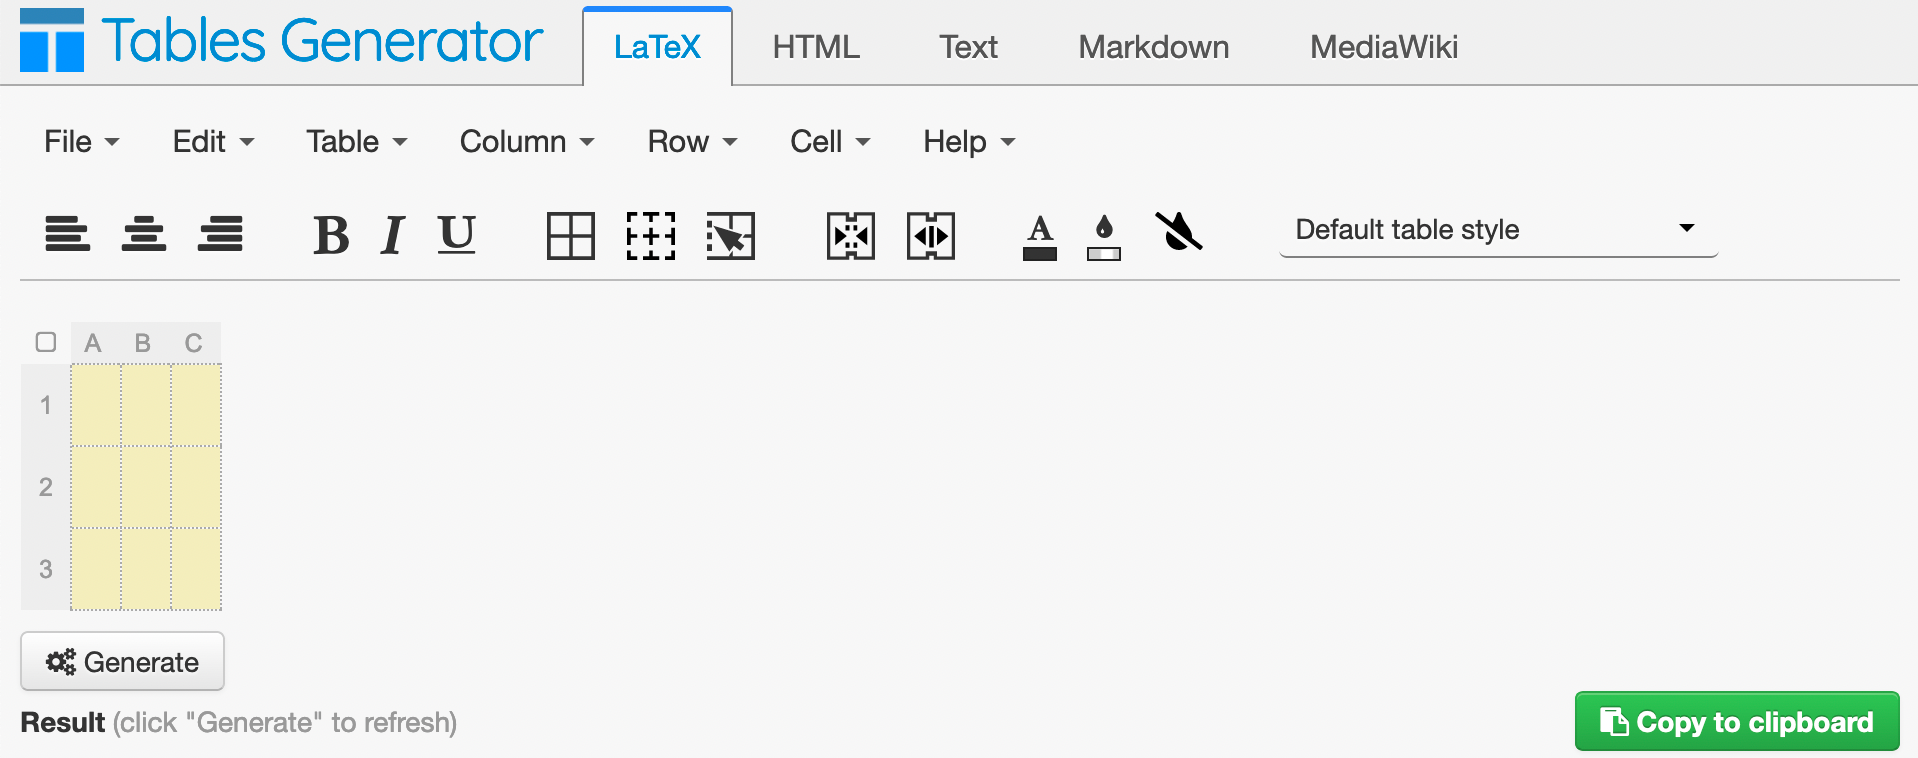
\includegraphics[width=\linewidth]{img/table_editor_300ppi.png}
	\caption{Página principal del editor de tablas en línea.}
	\label{fig:table_editor}
\end{figure}

El primer paso para generar una tabla es comprobar que estamos trabajando en la pestaña de \LaTeX{}. Posteriormente, para lograr una tabla de $3\times3$ como se ve en la figura \ref{fig:table_editor}, se selecciona \opcionMenu{File $\rightarrow$ New table...} y se introducen los valores para filas y columnas en la nueva pantalla (figura \ref{fig:new_table}).

\begin{figure}[ht!]
	\centering
	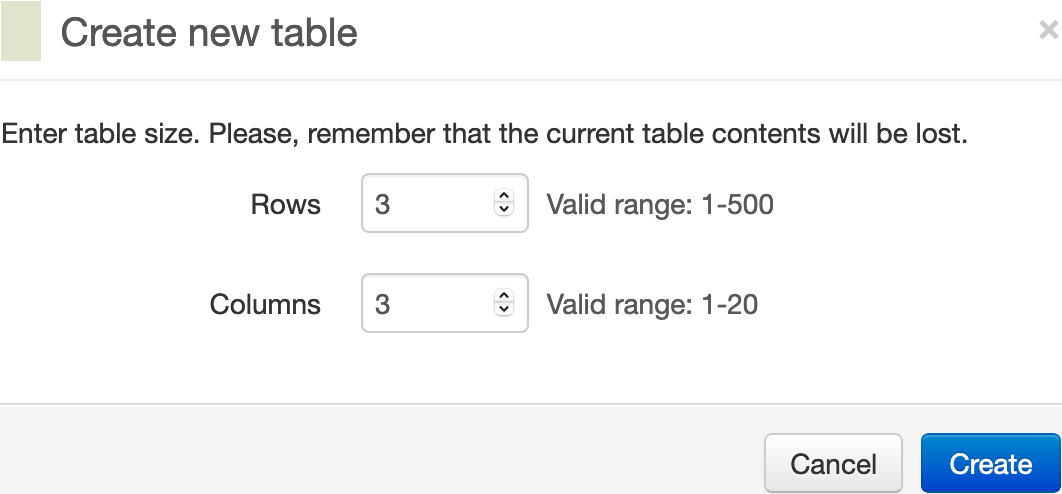
\includegraphics[scale=0.80]{img/table_new_table_300ppi.png}
	\caption{Diálogo modal para nuevas tablas.}
	\label{fig:new_table}
\end{figure}

En la cuadrícula podemos rellenar cada una de las celdas dando clic sobre ellas para escribir el contenido. Posteriormente, se le puede dar formato. De momento, introduce los valores que se ven en la figura \ref{fig:table_gatito}, simulando una partida de \emph{gato}.

\begin{figure}[ht!]
	\centering
	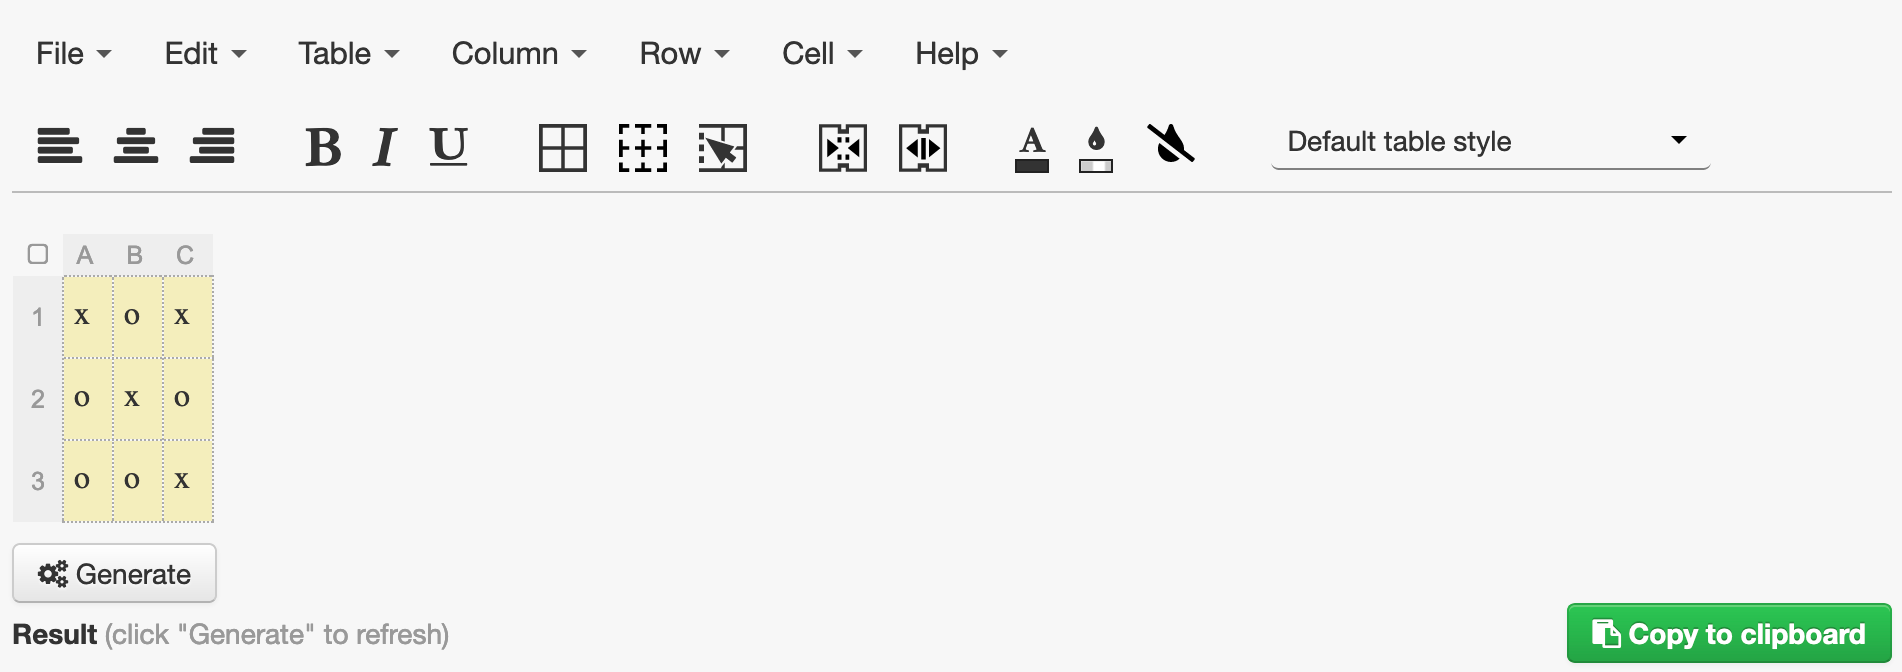
\includegraphics[width=\linewidth]{img/table_gatito_300ppi.png}
	\caption{Contenido de nuestro primer ejemplo de tabla.}
	\label{fig:table_gatito}
\end{figure}

Tras introducir el contenido damos clic en el botón \opcionMenu{Generate}, ubicado debajo de la tabla que editamos, para generar el código \LaTeX{}, mismo que se ve en la figura \ref{fig:table_gatito_codigo}. Además, puedes copiar todo el código generado gracias al botón \opcionMenu{Copy to clipboard} en el lado derecho, para así colocarlo en Overleaf.

\begin{figure}[ht!]
	\centering
	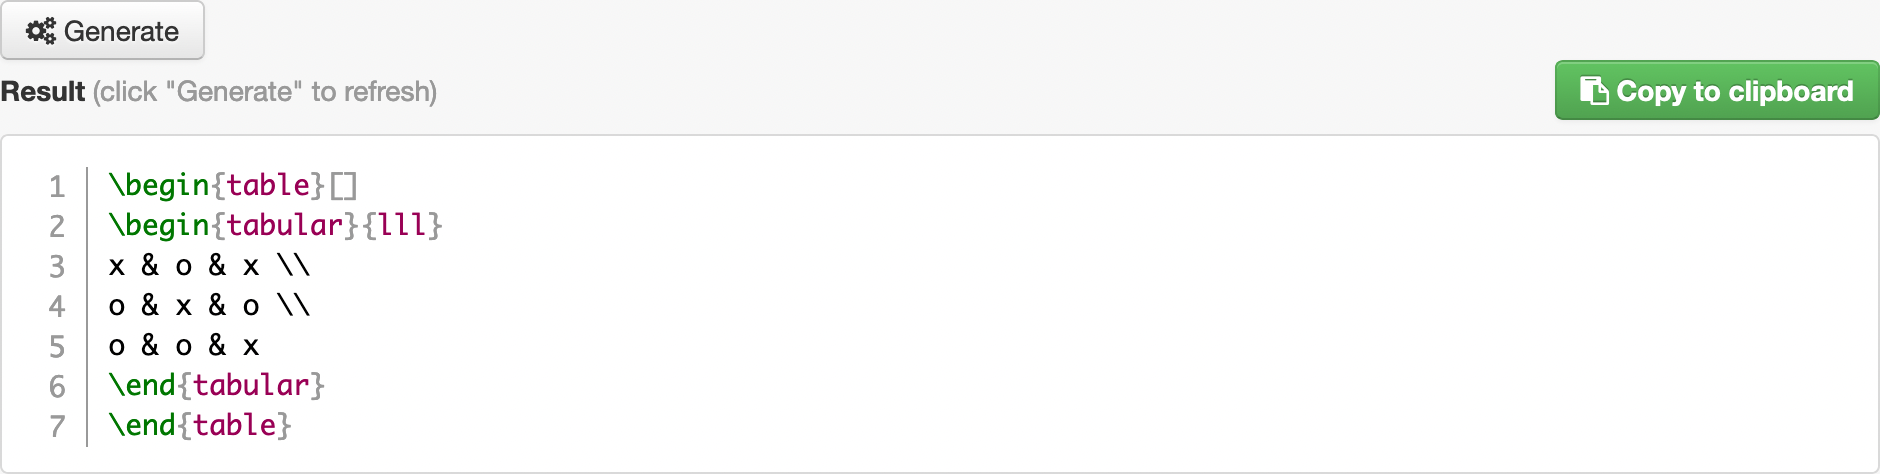
\includegraphics[width=\linewidth]{img/table_gatito_codigo_300ppi.png}
	\caption{Código generado para nuestro primer ejemplo de tabla.}
	\label{fig:table_gatito_codigo}
\end{figure}

Ahora que hemos llegado al código generado, el resto del capítulo tendrá el código en listados para explicar las líneas relevantes, aunque dicho código proviene del editor en línea. Lo primero que tenemos que revisar es el entorno \texttt{table}.


\section{Entorno \texttt{table}}
\label{sec:entorno_table}


El código generado por el editor se muestra en el listado \ref{lst:primera_tabla}. Y, sí, en esta página puede que veas un ``gatito'' perdido en la esquina superior izquierda, ¿qué pasó?

Si recuerdas la sección de elementos flotantes (página \pageref{sub:elementos_flotantes}), mencioné que la tabla pertencía a esta categoría. Y justo la primera línea de la tabla generada en el listado \ref{lst:primera_tabla} muestra el indicador de posición en unos corchetes vacíos al crear un entorno \texttt{table}.

\begin{lstlisting}[style=latex,caption={Código de primera tabla generada.},label=lst:primera_tabla]
\begin{table}[]
	\begin{tabular}{lll}
	x & o & x \\
	o & x & o \\
	o & o & x
	\end{tabular}
\end{table}
\end{lstlisting}

\begin{table}[]
	\begin{tabular}{lll}
	x & o & x \\
	o & x & o \\
	o & o & x
	\end{tabular}
\end{table}

Como no existe el indicador \texttt{!}, ni el \texttt{h}, lo que sigue en la prioridad es una \texttt{t}, para ubicar el elemento flotante (el entorno \texttt{table}) en la parte superior de la página. Como también carecemos de la instrucción ^\centering^, la tabla aparece alineada a la izquierda, la posición predeterminada del texto en idioma español.

Para terminar, la tabla carece de una leyenda y, por lo tanto, de una etiqueta que nos permita hacer referencias posteriormente. En conclusión, una tabla puede tener los mismos cuatro elementos que la figura:
\begin{enumerate}
	\item Indicador de ubicación \texttt{ht!}, para ubicarla cerca de su posición en el código.
	\item La instrucción ^\centering^, para centrarla horizontalmente.
	\item Una leyenda para describir su propósito.
	\item Una etiqueta, para usar de referencia.
\end{enumerate}

El editor en línea tiene opciones adicionales para agregar casi todo lo anteriormente mencionado, pero primero acabaremos la explicación del código que ya tenemos.



\section{Entorno \texttt{tabular}}
\label{sec:entorno_tabular}



De la misma forma en la que el entorno \texttt{figure} solo envolvía un \texttt{picture} o un ^\includegraphics^, el entorno \texttt{table} sirve solamente para generar la leyenda y la etiqueta, pero la acción de verdad pasa en el entorno \texttt{tabular}.

El entorno \texttt{tabular} comienza en la segunda línea en el listado \ref{lst:primera_tabla}, y recibe un argumento obligatorio (el valor entre llaves) que determina la alineación de cada una de las columnas presentes en la tabla.

Es decir, si decides eliminar por completo este argumento, dejando solamente

\begin{lstlisting}[style=latex,numbers=none]
\begin{tabular}
\end{lstlisting}

\noindent tendrás bastantes errores con los cuales lidiar:

\begin{lstlisting}[style=errores]
LaTeX Error: Illegal character in array arg. [	x]
Extra alignment tab has been changed to \cr. [	x &]
Extra alignment tab has been changed to \cr. [	x & o &]
Extra alignment tab has been changed to \cr. [	o &]
Extra alignment tab has been changed to \cr. [	o & x &]
Extra alignment tab has been changed to \cr. [	o &]
Extra alignment tab has been changed to \cr. [	o & o &]
\end{lstlisting}

Sí, todo un desastre aunque solo quitamos el argumento requerido para el entorno \texttt{tabular}. Únicamente recuerda: si en alguna tabla tienes errores similares, siempre revisa que el argumento esté presente.

No obstante, su sola presencia no basta porque tiene que coincidir con el número de columnas. De lo contrario, si dejamos solamente dos (en este ejemplo), con

\begin{lstlisting}[style=latex,numbers=none]
\begin{tabular}{ll}
\end{lstlisting}

\noindent aún tenemos una parte de los errores que salieron cuando removimos completamente el argumento:

\begin{lstlisting}[style=errores]
Extra alignment tab has been changed to \cr. [	x & o &]
Extra alignment tab has been changed to \cr. [	o & x &]
Extra alignment tab has been changed to \cr. [	o & o &]
\end{lstlisting}

De cualquier forma, el generador hace el conteo de columnas por nosotros y coloca bien la cantidad, así que este conocimiento nos es útil para modificar después si es necesario. Tres columnas, tres letras...

¿Pero por qué \texttt{l}? Para especificar alineación a la izquierda, del inglés \emph{left}. Podemos usar al menos los siguientes tres valores:
\begin{itemize}
	\item \texttt{l}, para alinear a la izquierda,
	\item \texttt{c}, para alinear al centro, y
	\item \texttt{r}, del inglés \emph{right}, para alinear a la derecha.
\end{itemize}

Lo que resta de contenido, las líneas:

\begin{lstlisting}[style=latex,numbers=none]
x & o & x \\
o & x & o \\
o & o & x
\end{lstlisting}

\noindent corresponden a cada una de las filas en la tabla, con cada una de sus tres columnas. ¿Cómo separamos una línea de la otra? Con la instrucción \codigo{\textbackslash{}} al final de la línea. ¿Y cómo se separan las columnas? Con el símbolo \texttt{\&}.

Al editar tablas manualmente tenemos que garantizar que la cantidad de \emph{ampersand} (\texttt{\&}) por fila sea de \texttt{columnas - 1} (se necesitan dos ampersand parar generar tres columnas), y que el argumento del entorno \texttt{tabular} contenga \texttt{columnas} indicadores de alineación (tres columnas, tres letras de alineación).



\section{Generador: opciones adicionales}
\label{sec:generador_opciones_adicionales}



Podemos agregarle a una tabla los mismos elementos que a una figura, desde el generador en línea. Debajo del código producido existe un pequeño \emph{combobox}\footnote{Elemento de la interfaz con una flechita a la derecha, que permite seleccionar varias opciones.} que permite agregar la leyenda y la instrucción de centrado (figura \ref{fig:table_editor_extra_options}). Siguiendo con el formato del libro, colocaremos la leyenda debajo, seleccionando \opcionMenu{Caption below}, y agregaremos la instrucción de centrado horizontal eligiendo \opcionMenu{Center table horizontally}.

\begin{figure}[ht!]
	\centering
	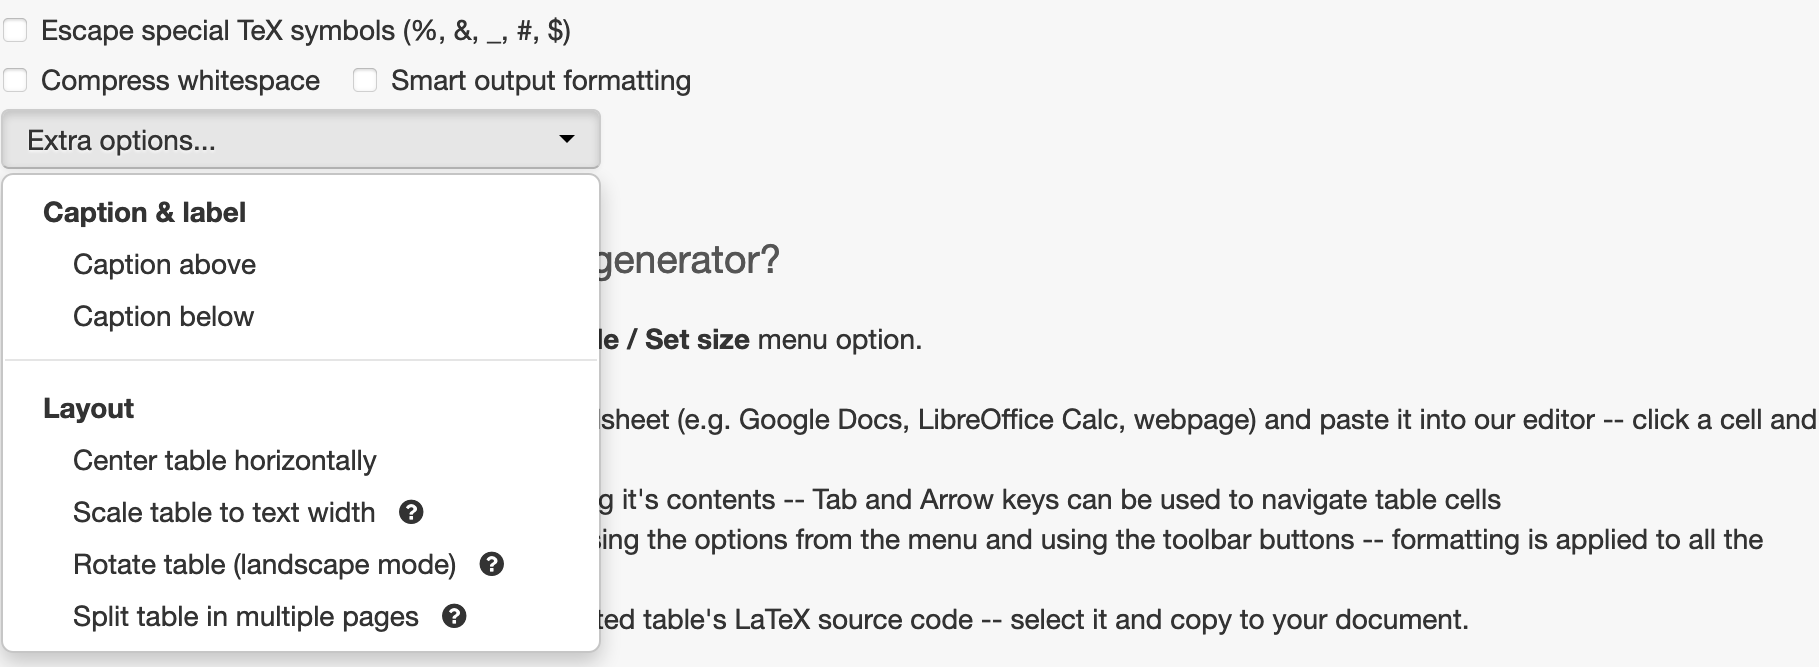
\includegraphics[width=\linewidth]{img/table_editor_extra_options_300ppi.png}
	\caption{Opciones adicionales para la tabla.}
	\label{fig:table_editor_extra_options}
\end{figure}

Tras seleccionar estas dos opciones, el \emph{combobox} se actualizará al valor \texttt{Caption below, center table horizontally}, y agregará dos cajas de texto a la interfaz, sobre el código: una para colocar la leyenda (caja de \texttt{Table caption}) y otra para la etiqueta (caja de \texttt{label}). La interfaz actualiza tras estos cambios se muestra en la figura \ref{fig:table_editor_caption}.

\begin{figure}[ht!]
	\centering
	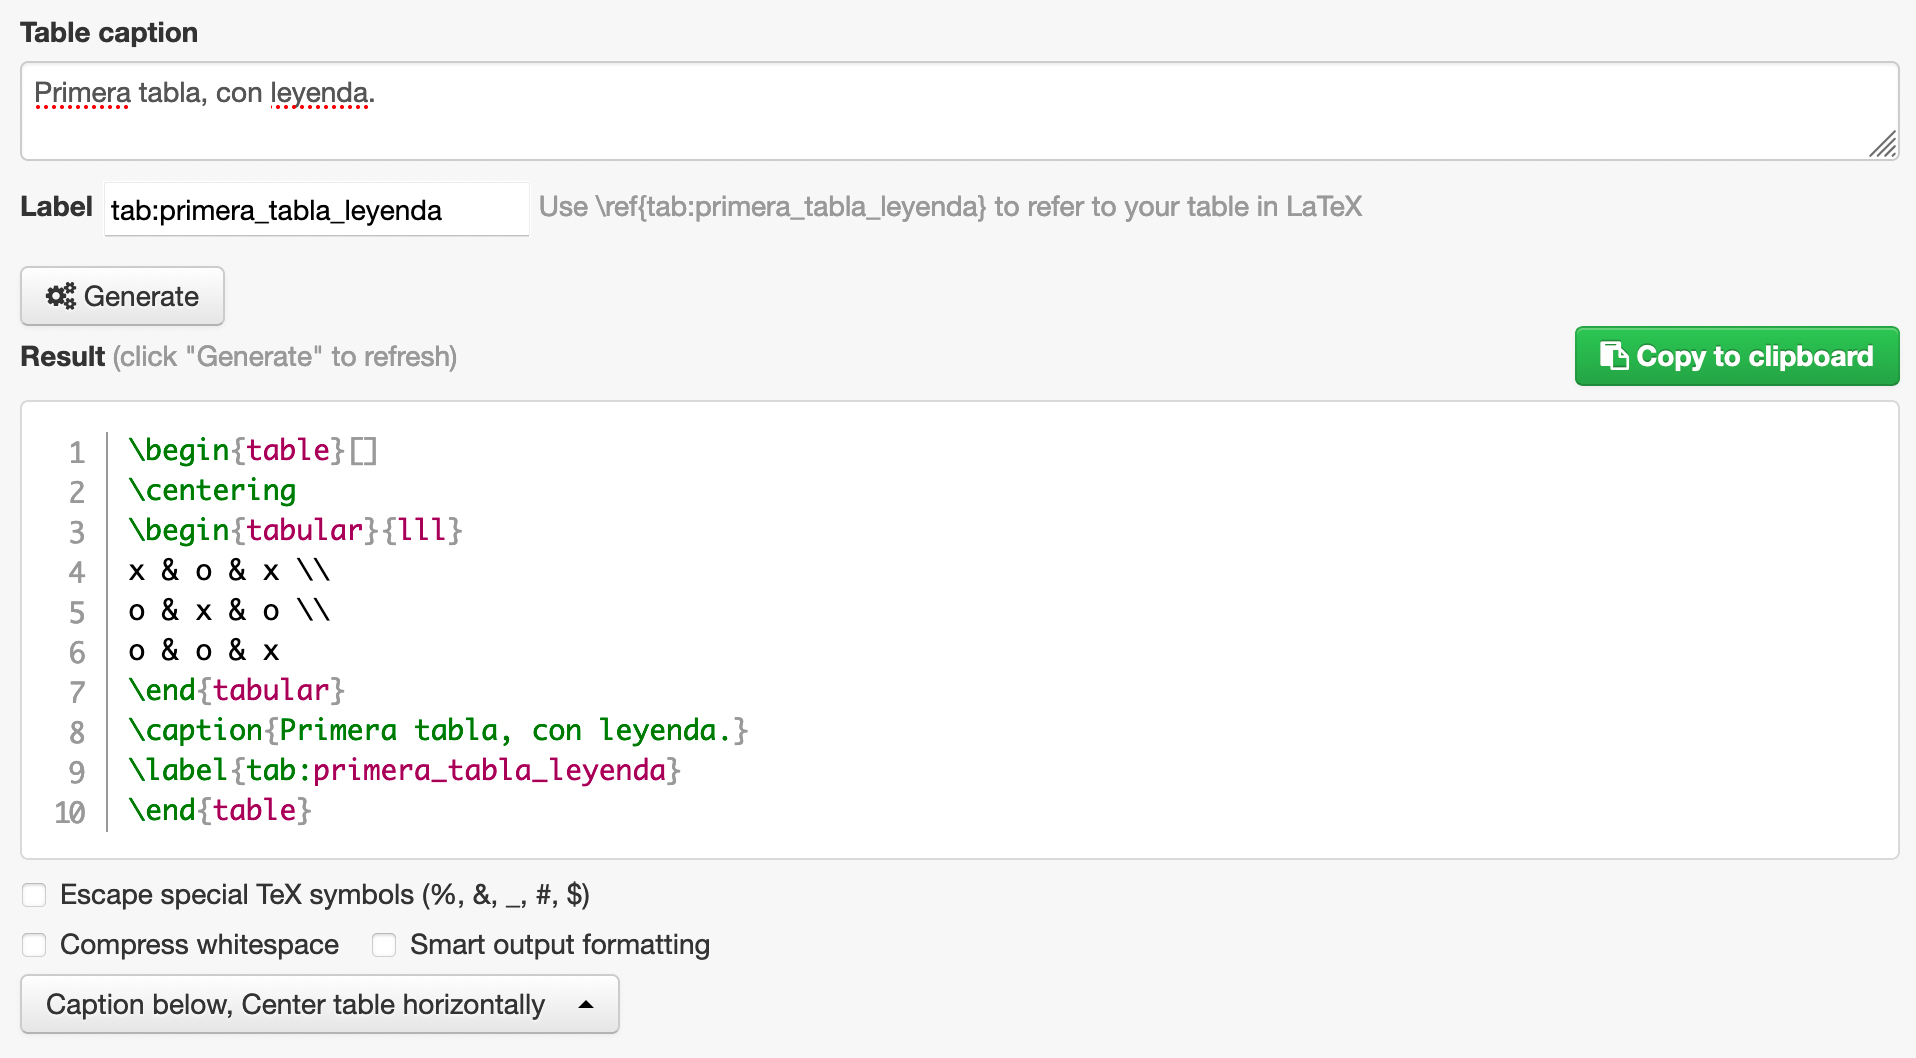
\includegraphics[width=\linewidth]{img/table_editor_caption_300ppi.png}
	\caption{Caja de texto para introducir leyenda y etiqueta.}
	\label{fig:table_editor_caption}
\end{figure}

Lo único que el generador no permite agregar es el indicador de ubicación, el valor entre corchetes del entorno \texttt{table}. No obstante, como se comporta de manera similar a una figura, utilizamos el indicador \texttt{ht!}. El código nuevo generado, más la ubicación de la tabla, se muestra en el listado \ref{lst:tabla_leyenda}.

\begin{lstlisting}[style=latex,caption={Código para tabla con leyenda.},label=lst:tabla_leyenda]
\begin{table}[ht!]
	\centering
	\begin{tabular}{lll}
		x & o & x \\
		o & x & o \\
		o & o & x
	\end{tabular}
	\caption{Primera tabla, con leyenda.}
	\label{tab:primera_tabla_leyenda}
\end{table}
\end{lstlisting}

Dado que ya tiene una leyenda y una etiqueta, podemos referenciar la tabla mediante un ^\ref{tab:primera_tabla_leyenda}^, similar a una figura. Por lo tanto, ya podemos decir que el código del listado \ref{lst:tabla_leyenda} da como resultado la tabla \ref{tab:primera_tabla_leyenda}.

\begin{table}[ht!]
	\centering
	\begin{tabular}{lll}
		x & o & x \\
		o & x & o \\
		o & o & x
	\end{tabular}
	\caption{Primera tabla con leyenda.}
	\label{tab:primera_tabla_leyenda}
\end{table}



\section{Bordes}
\label{sec:bordes}



Ya que tenemos el contenido, ¿dónde está la rejilla que me permite saber que estoy jugando gato? ¿Cómo colocamos los bordes de las celdas?

Esto tiene dos respuestas, porque depende si quieres bordes entre columnas o bordes entre filas. Para colocar los bordes entre columnas se utiliza el símbolo de línea vertical (\texttt{|}) junto con el argumento de la alineación del entorno \texttt{tabular}. Es decir, si queremos borde entre las columnas 1 y 2, y entre las columnas 2 y 3, el nuevo valor de dicho algumento es \texttt{\{l | l | l\}} (con espacios solo para mejor estética en el código).

Pero si queremos una línea que separe las filas 1 y 2, y las filas 2 y 3, es necesario usar la instrucción ^\hline^ al terminar el renglón. El código del listado \ref{lst:tabla_bordes} genera la tabla que se muestra en la columna derecha:

\noindent \begin{minipage}[ht!]{.80\linewidth}
% Aparentemente, no se pueden meter floats a un minipage,
% por eso no puedo tener mi table dentro de estas dos columnas.
\begin{lstlisting}[style=latex,frame={},caption={Código de tabla con bordes.},label=lst:tabla_bordes]
\begin{tabular}{l|l|l}
	x & o & x \\ \hline
	o & x & o \\ \hline
	o & o & x
\end{tabular}
\end{lstlisting}
\end{minipage}
\begin{minipage}[ht!]{.19\linewidth}
\begin{center}
	\vspace{-0.7cm}
	\begin{tabular}{l|l|l}
		x & o & x \\ \hline
		o & x & o \\ \hline
		o & o & x
	\end{tabular}
\end{center}
\end{minipage}

No obstante, ¿qué pasa si no queremos un borde que cubra de lado a lado, o de arriba a abajo, completamente? En el caso de las filas, sustituimos la instrucción ^\hline^ por una ^\cline^, seguida del rango de columnas que tendrá borde.

Por ejemplo, digamos que queremos que el borde inferior de la primera fila del gato cubra únicamente las columnas 1 y 2, y el borde inferior de la segunda fila solo las columnas 1 y 3. En el primer caso, una instrucción ^\cline{1-2}^ cubrirá lo necesario, pero para el segundo caso serán necesarias dos instrucciones separadas: ^\cline{1-1}^ y ^\cline{3-3}^ (nótese que se utiliza un rango aunque la línea vaya a cubrir una sola celda).

La tabla con estos nuevos bordes se crea en el listado \ref{lst:table_uneven_row_borders}, aunque también se puede generar con el editor en línea seleccionando los bordes deseados con la opción \opcionMenu{Custom Grid Edit}, botón que se encuentra resaltado en naranja en la figura \ref{fig:table_borders}. Ya eligirás tú si prefieres escribir el código o dar clic en los bordes correspondientes.

\begin{figure}[ht!]
	\centering
	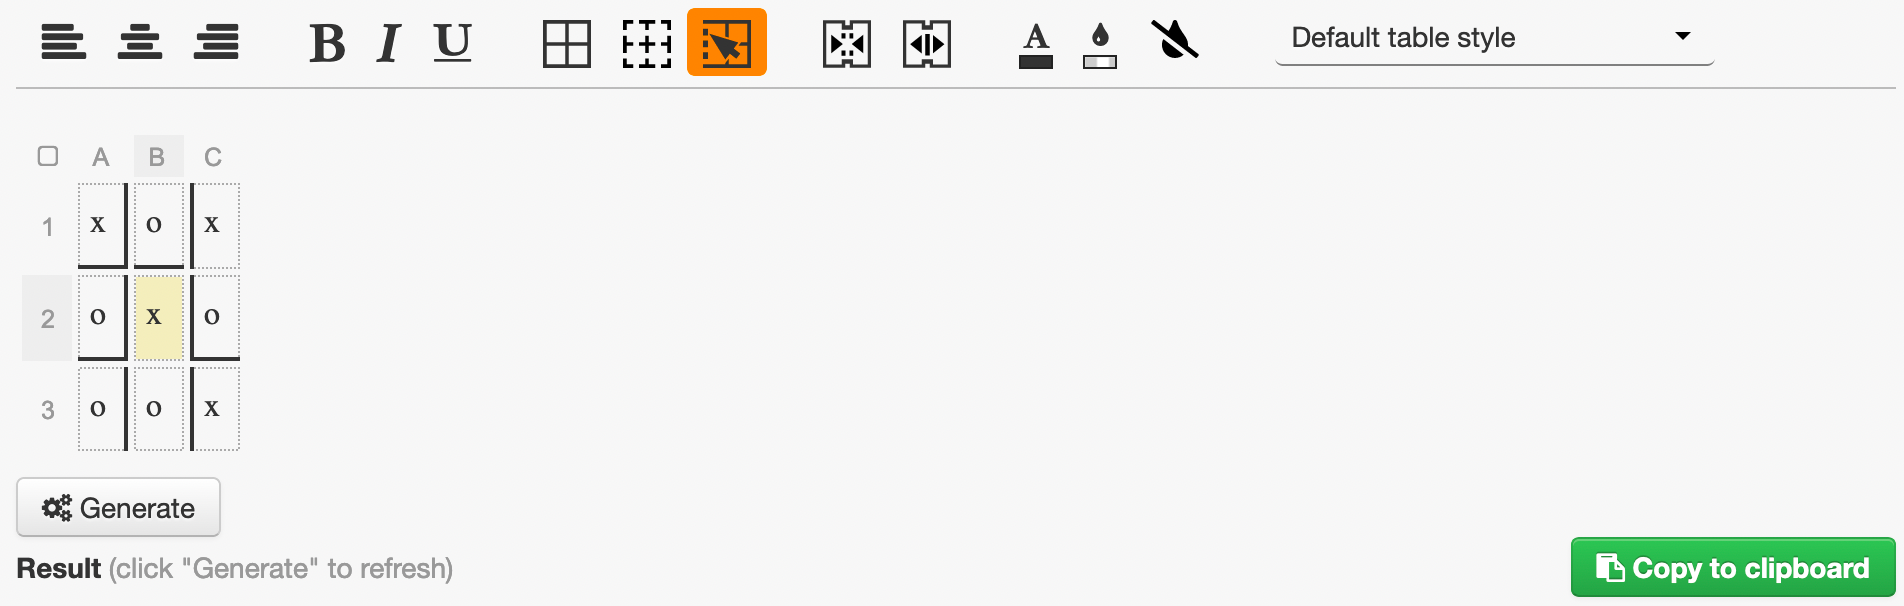
\includegraphics[width=\linewidth]{img/table_borders_300ppi.png}
	\caption{Edición de bordes con editor en línea.}
	\label{fig:table_borders}
\end{figure}

\noindent \begin{minipage}[ht!]{.80\linewidth}
\begin{lstlisting}[style=latex,frame={},caption={Código de tabla con bordes incompletos para filas.},label=lst:table_uneven_row_borders]
\begin{tabular}{l|l|l}
	x & o & x \\ \cline{1-2}
	o & x & o \\ \cline{1-1} \cline{3-3}
	o & o & x
\end{tabular}
\end{lstlisting}
\end{minipage}
\begin{minipage}[ht!]{.19\linewidth}
\begin{center}
	\vspace{-0.7cm}
	\begin{tabular}{l|l|l}
		x & o & x \\ \cline{1-2}
		o & x & o \\ \cline{1-1} \cline{3-3} 
		o & o & x
	\end{tabular}
\end{center}
\end{minipage}

¿Cómo colocamos bordes a solo una parte de la columna? En términos del generador en línea, sigue siendo cosa de manualmente elegir con el ratón cada borde. En código... es una nueva instrucción por cada celda con borde entre columnas.

Lo primero que hay que hacer para establecer bordes laterales parciales es remover el borde del indicador del entorno \texttt{tabular}. Después de eso, cada celda con borde lateral debe ser sustituida de su simple contenido (la \texttt{o} u \texttt{x} en el ejemplo) a una instrucción ^\multicolumn^ con el siguiente formato:

\begin{lstlisting}[style=latex,numbers=none]
\multicolumn{1}{alineación y bordes}{contenido}
\end{lstlisting}

Por ejemplo, si en la primera fila queremos conservar solamente el borde a la derecha de la \texttt{o}, sustituimos con un ^\multicolumn{1}{l|}{o}^ (si fuera a la izquierda, sería un ^\multicolumn{1}{|l}{o}^). En la segunda fila no habrá bordes, y en la tercera línea colocamos bordes a ambos lados de la \texttt{o} central. El código generado se muestra en el listado \ref{lst:table_uneven_col_borders}.

\noindent \begin{minipage}[ht!]{.80\linewidth}
\begin{lstlisting}[style=latex,frame={},caption={Código de tabla con bordes incompletos para columnas.},label={lst:table_uneven_col_borders}]
\begin{tabular}{lll}
x                      & \multicolumn{1}{l|}{o} & x \\
\cline{1-2}
o                      & x                      & o \\
\cline{1-1} \cline{3-3}
\multicolumn{1}{l|}{o} & \multicolumn{1}{l|}{o} & x
\end{tabular}
\end{lstlisting}
\end{minipage}
\begin{minipage}[ht!]{.19\linewidth}
\begin{center}
	\vspace{-0.7cm}
	\begin{tabular}{lll}
		x                      & \multicolumn{1}{l|}{o} & x \\ \cline{1-2}
		o                      & x                      & o \\ \cline{1-1} \cline{3-3} 
		\multicolumn{1}{l|}{o} & \multicolumn{1}{l|}{o} & x
	\end{tabular}
\end{center}
\end{minipage}

Sí, sé que te lo preguntas: ¿por qué el generador puso los bordes en dos celdas distintas si pudimos haber puesto los dos bordes sobre una misma celda? Como quizá sospechas, las instrucciones

\begin{lstlisting}[style=latex,numbers=none]
\multicolumn{1}{l|}{o} & \multicolumn{1}{l|}{o} & x
\end{lstlisting}

\noindent y

\begin{lstlisting}[style=latex,numbers=none]
o & \multicolumn{1}{|l|}{o} & x
\end{lstlisting}

\noindent son equivalentes. Ya será cuestión de preferencias el cómo decides redactar el código, mientras el objetivo se logre.


\section{Centrado de encabezados}
\label{sec:centrado_de_encabezados}



Para el centrado de encabezados se utiliza la misma instrucción que para colocar bordes individuales: ^\multicolumn^. Para centrar, o cambiar la alineación respecto al parámetro global del \texttt{tabular}, se utiliza el indicador de alineación. Por ejemplo, para la tabla \ref{tab:instrucciones_de_secciones} (pp.\pageref{tab:instrucciones_de_secciones}) se utilizó el código que se muestra en el listado \ref{lst:table_ubicacion}.

\begin{lstlisting}[style=latex,numbers=left,caption={Código de tabla de indicadores de ubicación.},label={lst:table_ubicacion},
linebackgroundcolor={%
	\ifnum \value{lstnumber} =  5 \color{codigo_linea_resaltada}
	\else \color{codigo_fondo}
	\fi % Tantos \fi como líneas subrayadas.
}]
\begin{table}[ht]
\centering
\begin{tabular}{cl}
\hline
\textbf{Parámetro} & \multicolumn{1}{c}{\textbf{Posición}}
\\
\hline
\texttt{h}         & Aquí... por favor, y si es posible.                           \\
\texttt{t}         & En la parte superior de la página (del inglés \emph{top}).    \\
\texttt{b}         & En la parte inferior de la página (del inglés \emph{bottom}). \\
\texttt{p}         & Colocar en una página especial para flotantes.                \\
\texttt{!}         & Ignorar los parámetros que \LaTeX{} considera buenos.         \\
\texttt{H}         & Sin comentarios...                                            \\
\hline
\end{tabular}
\caption{Posibles valores del indicador de ubicación.} % Leyenda de la tabla.
\label{tab:indicador_ubicacion}
\end{table}
\end{lstlisting}

La línea de nuestro interés en el listado \ref{lst:table_ubicacion} es la 5,

\begin{lstlisting}[style=latex,numbers=none]
\textbf{Parámetro} & \multicolumn{1}{c}{\textbf{Posición}}
\end{lstlisting}

\noindent donde se utiliza la instrucción ^\multicolumn^ para producir el título \emph{Posición} centrado, con el resto del contenido en la columna alineado a la izquierda. El segundo par de llaves en esa instrucción es lo que nos interesa. Tuvimos que escribir todo el ^\multicolumn^, con sus tres pares de llaves, solo para cambiar una \texttt{l}, definida en el entorno \texttt{tabular}, por una \texttt{c}, definida a nivel celda.

Aprovechando la ocasión del desastre que parece el listado \ref{lst:table_ubicacion}, hablemos de uno de los problemas de editar tablas en \LaTeX{}: editar a mano es un dolor de cabeza por el espacio en blanco. En el listado, las líneas 8, 9, 10... bueno, todas las líneas con contenido en los renglones tuvieron que expandirse a dos debido a su longitud por espacio en blanco. No obstante, al editar sin separar las líneas por ancho de página, el código luce como en la figura \ref{fig:codigo_tabla_espacio}, con un orden visual tranquilizador.

El problema es que, con solo dos columnas, ya ocupamos casi todo el espacio disponible para una línea en el monitor, gracias a los encabezados centrados que demandan tanto espacio en términos de caracteres... pero la opción es editar sin alinear columnas y tener que buscar los ampersand para saber dónde tenemos que editar a mano.

De cualquier forma, pierdes: o tienes mucho espacio vacío y la necesidad de usar barra desplazadora, o tienes todo compacto pero sin un apoyo visual que te diga dónde están las columnas. O lo peor de ambos mundos\footnote{Te he fallado, Hannah Montana :(.}, lo que ocurrió en el listado \ref{lst:table_ubicacion} por su necesidad de ser una página impresa: mucho espacio vacío, con líneas separadas para no exceder los márgenes del documento, lo que te quita la habilidad de ver fácilmente dónde están las columnas.

\begin{figure}[ht!]
	\centering
	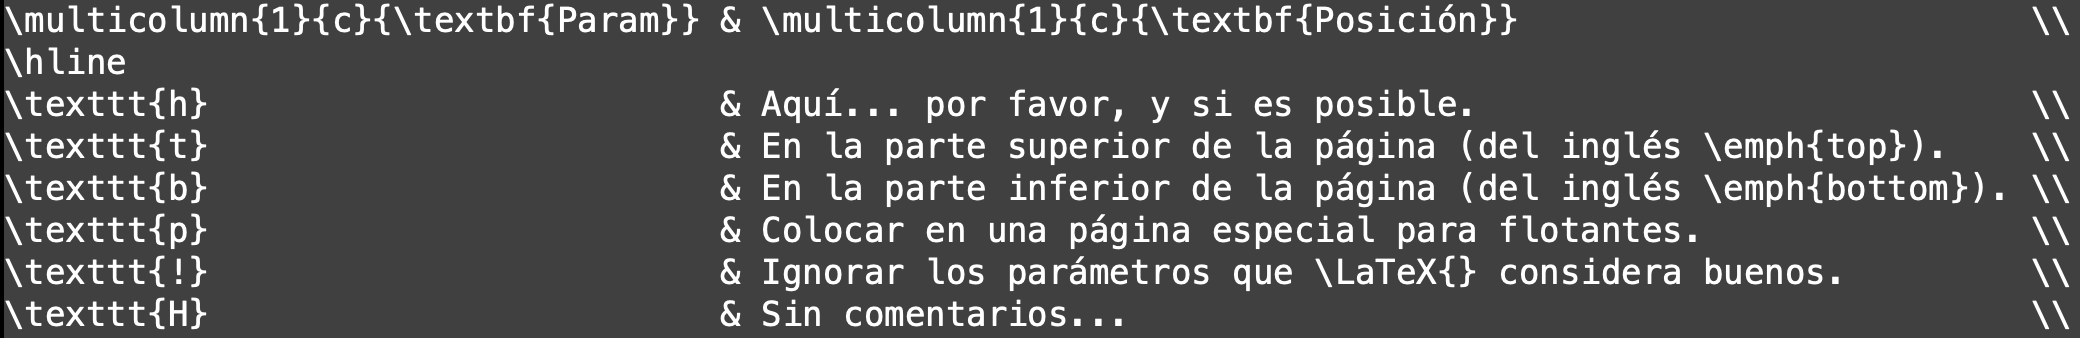
\includegraphics[width=\linewidth]{img/table_code_space.png}
	\caption{Editando código de tabla en ancho fijo, sin separar líneas.}
	\label{fig:codigo_tabla_espacio}
\end{figure}



\section{Combinación de columnas}
\label{sec:combinacion_de_columnas}



Después de haberla utilizado para bordes y centrar un encabezado, por fin vamos a darle el uso legítimo a la instrucción ^\multicolumn^. Resulta que se llama así porque sirve para hacer que una celda se expanda a múltiples columnas (del inglés \emph{multiple column}). Unir celdas horizontalmente, pues. Y, sí, justo ese primer parámetro, ese \texttt{1} olvidado, es la cantidad de columnas que esta nueva multicolumna debe abarcar dentro de la fila.

\begin{table}[ht]
\centering
\begin{tabular}{l|rrr}
\hline
\multicolumn{4}{c}{\textbf{Calificaciones de 4A}} \\ \hline
Carlos         & 4         & 8         & 4        \\
Ixchel         & 10        & 9         & 8        \\
Abimael        & 9         & 10        & 10       \\ \hline
\end{tabular}
\caption{Tabla con columnas unidas.}
\label{tab:calificaciones}
\end{table}

La tabla \ref{tab:calificaciones} tiene un encabezado que se expande a lo largo de las cuatro columnas, longitud que se indica en la línea 5 del listado \ref{lst:tabla_calificaciones} con el primer parámetro entre llaves. En esta línea ya no utilizamos más ampersands\footnote{Sí, en español se supone que se llama \textbf{et}... la costumbre.} (\&) porque la multicolumna se encarga de representar todas las columnas.

\begin{lstlisting}[style=latex,numbers=left,caption={Tabla con encabezado de cuatro columnas de ancho.},label={lst:tabla_calificaciones},
linebackgroundcolor={%
	\ifnum \value{lstnumber} =  5 \color{codigo_linea_resaltada}
	\else \color{codigo_fondo}
	\fi % Tantos \fi como líneas subrayadas.
}]
\begin{table}[ht]
\centering
\begin{tabular}{l|rrr}
\hline
\multicolumn{4}{c}{\textbf{Calificaciones de 4A}} \\ \hline
Carlos         & 4         & 8         & 4        \\
Ixchel         & 10        & 9         & 8        \\
Abimael        & 9         & 10        & 10       \\ \hline
\end{tabular}
\caption{Tabla con columnas unidas.}
\label{tab:calificaciones}
\end{table}
\end{lstlisting}



\section{Combinación de filas	}
\label{sec:combinacion_de_filas}


Supongamos ahora que debemos incluir una tabla que necesita agrupar un conjunto de filas. Por ejemplo, la tabla \ref{tab:estados_norte} muestra un extracto de los estados de México agrupados por zona. ¿Cómo fue hecha?

\begin{table}[ht]
\centering
\begin{tabular}{ll}
\hline
\multicolumn{1}{c}{\textbf{Zona}} & \multicolumn{1}{c}{\textbf{Estado}}
\\ \hline
\multirow{4}{*}{Norte}            & Chihuahua                           \\
                                  & Durango                             \\
                                  & Coahuila                            \\
                                  & Nuevo León                          \\ \hline
\end{tabular}
\caption{Ejemplo de tabla con \texttt{multirow}.}
\label{tab:estados_norte}
\end{table}

Para la combinación de filas requerimos de un paquete adicional: \texttt{multirow}. Este paquete nos dará la habilidad de usar la instrucción ^\multirow^, que tiene un formato similar a ^\multicolumn^:

\begin{lstlisting}[style=latex,numbers=none]
\multirow{número de filas}{alto}{contenido de las celdas}
\end{lstlisting}

El listado \ref{lst:tabla_estados} nos muestra un ejemplo de tabla con celda multifila. La línea 7 crea una celda de cuatro filas de alto (según su primer parámetro) y tiene el contenido de \emph{Norte} (según el tercer par de llaves). La estrella (\texttt{*}) en el segundo parámetro sirve para indicarle al compilador que debe calcular automáticamente la altura de la celda en base a la cantidad de filas sobre las cuales se expande. Esto con el fin centrar verticalmente el contenido.

Pero, entonces, ¿cómo se cambia la alineación horizontal de una fila que se expande a lo alto de cuatro filas? Justo como lo hicimos para una sola celda, usando ^\multicolumn^. Si quieres más detalles sobre cómo utilizar una multicolumna con una multifila puedes consultar \cite{bib:multicol_multirow}.

\begin{lstlisting}[style=latex,numbers=left,caption={Tabla con columna de cuatro filas de alto.},label={lst:tabla_estados},
linebackgroundcolor={%
	\ifnum \value{lstnumber} =  7 \color{codigo_linea_resaltada}
	\else \color{codigo_fondo}
	\fi % Tantos \fi como líneas subrayadas.
}]
\begin{table}[ht]
\centering
\begin{tabular}{ll}
\hline
\multicolumn{1}{c}{\textbf{Zona}}&\multicolumn{1}{c}{\textbf{Estado}}
\\ \hline
\multirow{4}{*}{Norte} & Chihuahua  \\
                       & Durango    \\
                       & Coahuila   \\
                       & Nuevo León \\ \hline
\end{tabular}
\caption{Ejemplo de tabla con \texttt{multirow}.}
\label{tab:estados_norte}
\end{table}
\end{lstlisting}

También puedes modificar otras cosas estéticas de la tabla, como el ancho de los bordes o los colores de fondo. No obstante, hasta aquí llega lo básico que necesitas para tu tesis. Si requieres estos cambios en el formato de una tabla, consulta \cite{bib:overleaf_tables}.



\section*{Resumen}



En este capítulo vimos que la mejor forma de trabajar con las tablas en \LaTeX{} es dejando que un generador las haga por nosotros. Aún así, analizamos el código necesario para codificar tablas de manera manual, en el no-tan-deseado caso de tener que hacer modificaciones sin ayuda del generador.

Estos cambios incluyen modificar el contenido de la celda, cambiar la alineación, colocar bordes, crear celdas multicolumna, y celdas multifila.

Ahora que hemos visto cómo incluir tablas, viene algo que promete ser aún más divertido: ecuaciones.

\lstDeleteShortInline^
\lstMakeShortInline[style=latexi]|